% =====================================================================
%  IASTAM 6.0 -- Track 4, Problem 7
%  "Transmitting Information Rather Than Raw Data"
%  INTERIM PAPER
%
%  Compile: pdflatex twice (Overleaf: just press Recompile).
%  Figures resolve from ../code/results/ and ../docs/ via \graphicspath.
%
%  LABEL CONVENTION, used on every figure and number in this paper:
%    [REAL]   measured on Airbus imagery with our trained models
%    [SIM]    produced by our orbit/link simulator, driven by REAL detections
%    [LIT]    taken from published work, cited
%    [ASSUM]  a value we chose; all of these are swept in Section 7
% =====================================================================
\documentclass[10pt,a4paper]{article}

\usepackage[T1]{fontenc}
\usepackage[utf8]{inputenc}
\usepackage[margin=2.2cm]{geometry}
\usepackage{graphicx}
\usepackage{booktabs}
\usepackage{amsmath}
\usepackage{amssymb}
\usepackage{xcolor}
\usepackage{caption}
\usepackage{subcaption}
\usepackage{multirow}
\usepackage[hidelinks]{hyperref}
\usepackage{enumitem}

% figures/ holds copies so this folder compiles standalone on Overleaf;
% the other two paths let it also build in place from the live results.
\graphicspath{{figures/}{../code/results/}{../docs/}}

\definecolor{real}{RGB}{46,139,87}
\definecolor{sim}{RGB}{27,108,168}
\definecolor{lit}{RGB}{125,60,152}
\definecolor{warn}{RGB}{192,57,43}

\newcommand{\REAL}{\textcolor{real}{\footnotesize\textsf{[REAL]}}}
\newcommand{\SIM}{\textcolor{sim}{\footnotesize\textsf{[SIM]}}}
\newcommand{\LIT}{\textcolor{lit}{\footnotesize\textsf{[LIT]}}}
\newcommand{\ASSUM}{\textcolor{warn}{\footnotesize\textsf{[ASSUM]}}}
\newcommand{\warnbox}[1]{%
  \par\smallskip\noindent\fcolorbox{warn}{warn!4}{%
  \parbox{\dimexpr\linewidth-2\fboxsep-2\fboxrule}{\small #1}}\par\smallskip}

\captionsetup{font=small,labelfont=bf}
\setlist{nosep,leftmargin=*}

\title{\textbf{Transmitting Information Rather Than Raw Data}\\[2pt]
\large A confidence-aware level-of-detail encoder and a value-aware\\
multi-pass downlink scheduler for small satellites}

\author{IASTAM 6.0 --- Track 4, Problem 7\\
\small\texttt{github.com/oblhdj/iastam-p7-semantic-downlink}}

\date{Interim report --- 26 September 2026}

\begin{document}
\maketitle

\begin{abstract}
\noindent
A small satellite images far more ocean than its radio can carry: in our modelled day it
acquires 60{,}124 MB and has 210 MB of downlink, so $99.7\%$ of what it sees is
discarded. The conventional response is stronger image compression. We instead stop sending
images: ships are detected on board, and the link is spent on \emph{information about them},
graded by detector confidence and scheduled by value per byte. On 53{,}195 real Airbus tiles,
with a detector we trained and real orbit passes from an SGP4 propagator, the system delivers
$557\times$ less data than a bent pipe while reporting $68.5\%$ of all ships --- which is
\emph{100\% of what the satellite still knew after detection}. The downlink is therefore no
longer the binding constraint; the detector is. Under congestion the scheduler delivers
$2.26\times$ more ships than FIFO, and an exact dynamic program shows the greedy policy is
within $0.251\%$ of optimal at operational scale. We place equal weight on what the work does
\emph{not} show: an unfair baseline that once flattered us by ten points, an image-quality
setting we had adopted as free that costs four points of small-ship recall, and the fact that
over half of all reported loss traces to a cloud assumption resting on 21 real tiles.
\end{abstract}

% =====================================================================
\section{Problem and contributions}

An optical smallsat in low Earth orbit sees a ground station only a few minutes per pass. Our
modelled mission (Section~\ref{sec:setup}) has five passes per day over Sfax, 34 minutes of
contact, and a worst-case gap of 11.4 hours. Against that, the imager produces tens of gigabytes.
Every published approach we surveyed attacks the ratio by compressing pixels harder
\LIT. That preserves the picture and discards the budget.

We make two contributions.

\begin{description}
\item[C1 --- Confidence-aware level of detail.] The payload for a detected ship is chosen by how
  certain the detector is. Above a calibrated threshold, a ship costs 40 bytes of metadata; below
  it, it earns a $\sim$900-byte image chip; a coastal tile the detector may have misread is sent
  whole. Section~\ref{sec:lod}.
\item[C2 --- Value-aware multi-pass scheduling.] The downlink is a knapsack that refills each
  pass. Items are ordered by value per byte, truncated progressively when a pass runs short, and
  carried across passes when it does not. Section~\ref{sec:sched}.
\end{description}

A third element emerged from the work rather than the plan: the two loops are coupled. The
encoder reads the buffer state and spends fewer bytes per tile when the queue is deep
(Section~\ref{sec:queue}), which is what makes the system robust across load regimes it was never
tuned for.

% =====================================================================
\section{Experimental setup}\label{sec:setup}

\paragraph{Data \REAL.} 53{,}195 tiles of $768\times768$ px from the Airbus Ship Detection
Challenge, split 42{,}555 / 5{,}320 / 5{,}320. The set contains heavy near-duplication: $19.1\%$
of tiles have a twin, and a naive random split leaks 1{,}617 duplicate groups across the
train/test boundary. Our split is built on connected components of a verified duplicate graph and
leaks \textbf{zero} groups. Every number in this paper is computed on the held-out test split.

\paragraph{Detector \REAL.} YOLOv8n at 768 px, 12 epochs. Test mAP50 $=0.804$, precision $0.817$,
recall $0.729$; 10.7 ms/tile on an RTX 5060. Recall by size is $0.739$ / $0.958$ / $0.994$ for
small ($<32$ px) / medium / large, \emph{at a confidence cut-off of $0.05$}; at the operational
cut-off of $0.25$ small-ship recall is substantially lower, and we never quote the two together.

\paragraph{Orbit and link \SIM.} SGP4 propagation of a 500 km sun-synchronous orbit; ground
station at Sfax; S-band CubeSat budget with a $0.25$ share allocated to this payload. Five passes
per day, 34 minutes of contact, 11.4 h maximum gap, 210 MB of capacity per modelled day.

\paragraph{Workload \SIM\ from \REAL\ detections.} A day is assembled by drawing real tiles ---
with their real detections, real confidences and real false alarms --- into an assumed
operational context mix of 15\% cloud, 20\% ships, 5\% coast, 60\% open sea \ASSUM. Everything
\emph{inside} a tile is measured; only the mix and the daily tile count are chosen.

% =====================================================================
\section{On-board stages}

\subsection{A learned gate replaces the classical pre-filter}\label{sec:gate}

The plan called for a cheap classical stage to skip empty tiles before the detector. Measured on
real tiles it is not usable as a gate: it retains only $0.645$ of ships while discarding $17.7\%$
of empty tiles \REAL. We replaced it with a 47k-parameter CNN at 128 px.

\begin{table}[h]\centering\small
\caption{Gate vs.\ classical pre-filter at matched compute \REAL. Threshold chosen on the
\emph{validation} split and reported on test; the generalisation gap is $0.23$ points.}
\begin{tabular}{lccc}
\toprule
empty tiles dropped & classical filter & \textbf{learned gate} & gain \\
\midrule
17.7\% & 0.645 & \textbf{0.996} & $+35.1$ pts \\
41.9\% & 0.555 & \textbf{0.987} & $+43.2$ pts \\
58.1\% & 0.333 & \textbf{0.976} & $+64.3$ pts \\
\bottomrule
\end{tabular}
\end{table}

The gate costs $0.154$ ms/tile against the classical filter's $56.3$ ms --- $365\times$ cheaper
--- which matters in Section~\ref{sec:seams}.

\warnbox{\textbf{Bounding the claim.} Only $20.4\%$ of tiles in this dataset are empty, so a
\emph{perfect} gate could skip at most that share of detector calls. The measured saving is
$7$--$9\%$ of compute. This is a property of a ship-detection benchmark, whose tiles were selected
for being interesting; a real ocean swath is mostly empty, where the same gate would save far
more. We therefore report $7$--$9\%$ as a \emph{floor}, and treat the gate's \emph{safety}, not
its saving, as the result this dataset can establish.}

\subsection{Calibration, and where the rungs belong}\label{sec:calib}

The level-of-detail ladder branches on raw detector confidence, so the thresholds are only
meaningful if that confidence is a probability. It is not. Fitted on the validation split and
evaluated on test, the detector is \emph{under}-confident: it reports a mean score of $0.352$ and
is correct $0.408$ of the time. Isotonic regression reduces expected calibration error
$8.9\times$, from $0.0878$ to $0.0099$ \REAL\ (Figure~\ref{fig:calib}).

The consequence is concrete. A raw score of $0.9$ does not mean 90\% certainty --- it is far
stricter --- which is why the cheap 40-byte rung fired on only $3.1\%$ of predictions. The score
that actually means $p=0.9$ is $\mathbf{0.670}$, where the rung serves $21.7\%$. Re-cutting the
threshold is measured as strictly better at every load: at 160k tiles/day it gains $1.5$ points of
recall, saves $8.1\%$ of bytes, and reduces latency.

\begin{figure}[h]\centering
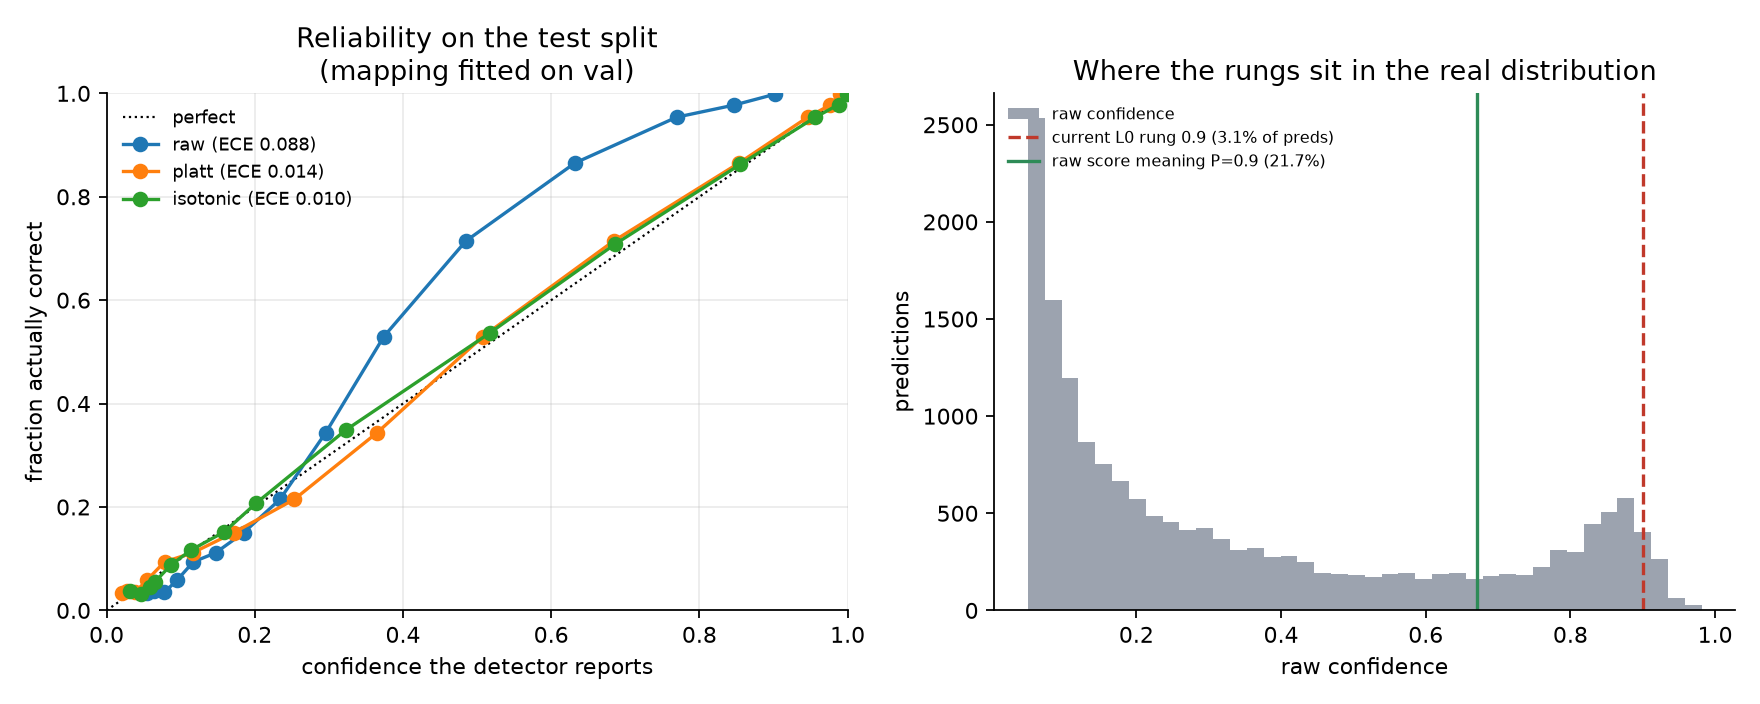
\includegraphics[width=0.82\textwidth]{wp2_reliability.png}
\caption{Reliability on the test split, with the mapping fitted on validation \REAL. Left:
the raw curve sits above the diagonal --- under-confidence. Right: where the rungs fall in the
real score distribution.}\label{fig:calib}
\end{figure}

\subsection{The level-of-detail encoder}\label{sec:lod}

Payload sizes are measured on 551 real ship crops and 300 real tiles \REAL, not assumed:

\begin{center}\small
\begin{tabular}{lrl}
\toprule
rung & bytes & content \\
\midrule
L0 & 40 & position, length, heading, confidence \\
L1 & $\sim$900 & tight image chip, q40 \\
L2 & $\sim$2{,}500 & region of interest including wake \\
coastal tile & 32{,}420 & the whole tile, q40 \\
thumbnail & $\sim$1{,}000 & safety net, 96 px \\
\bottomrule
\end{tabular}
\end{center}

Per-ship payload follows a power law fitted to the real crops, $\text{bytes}=137.5\,\ell^{0.57}$
for L1 and $43.3\,\ell^{1.14}$ for L2, with $\ell$ the ship's length in pixels.

\subsection{Value-aware scheduling}\label{sec:sched}

Each item $i$ carries a size $s_i$ and a value $v_i$; a pass with capacity $C$ is filled by
decreasing $v_i/s_i$, with progressive items truncated at the boundary. Dark vessels --- ships
without an AIS match \ASSUM\ --- carry $5\times$ weight. Section~\ref{sec:fmea} describes a defect
in that rule that we found only by injecting the fault.

% =====================================================================
\section{Results}\label{sec:results}

\begin{table}[h]\centering\small
\caption{Headline results \SIM\ over \REAL\ detections, 40{,}000 tiles/day. ``Ceiling'' is the
share of ships the satellite still knew about after detection and cloud gating --- the most any
downlink policy could deliver.}
\begin{tabular}{lrrrr}
\toprule
strategy & ship recall & ceiling & MB sent & reduction \\
\midrule
Bent pipe (raw, FIFO) & 0.002 & 0.841 & 201.7 & $298\times$ \\
Phi-sat-2 style, ocean only & 0.518 & 0.518 & 13.5 & --- \\
Phi-sat-2 style, \emph{fair} (+coastal) & 0.622 & 0.622 & 16.3 & --- \\
Ours: LoD + FIFO & 0.685 & 0.685 & 108.0 & $557\times$ \\
\textbf{Ours: LoD + value-greedy} & \textbf{0.685} & 0.685 & \textbf{108.0} & $\mathbf{557\times}$ \\
\bottomrule
\end{tabular}
\end{table}

Three readings matter, and they pull in different directions.

\begin{enumerate}
\item \textbf{At nominal load the downlink is not the bottleneck.} We deliver 100\% of what the
  satellite still knows. The gap from $1.0$ to $0.685$ is the detector and the cloud gate, not the
  link. Scheduling buys nothing here, and we say so.
\item \textbf{Scheduling pays only under congestion.} At 160k tiles/day the link saturates and
  value-greedy delivers $0.662$ against FIFO's $0.293$ --- $2.26\times$
  (Figure~\ref{fig:sweep}).
\item \textbf{Against a fair baseline the margin is modest.} $+6.3$ points at nominal load,
  $+4.1$ under congestion, for roughly $7\times$ the bytes of a fixed-patch scheme.
\end{enumerate}

\begin{figure}[h]\centering
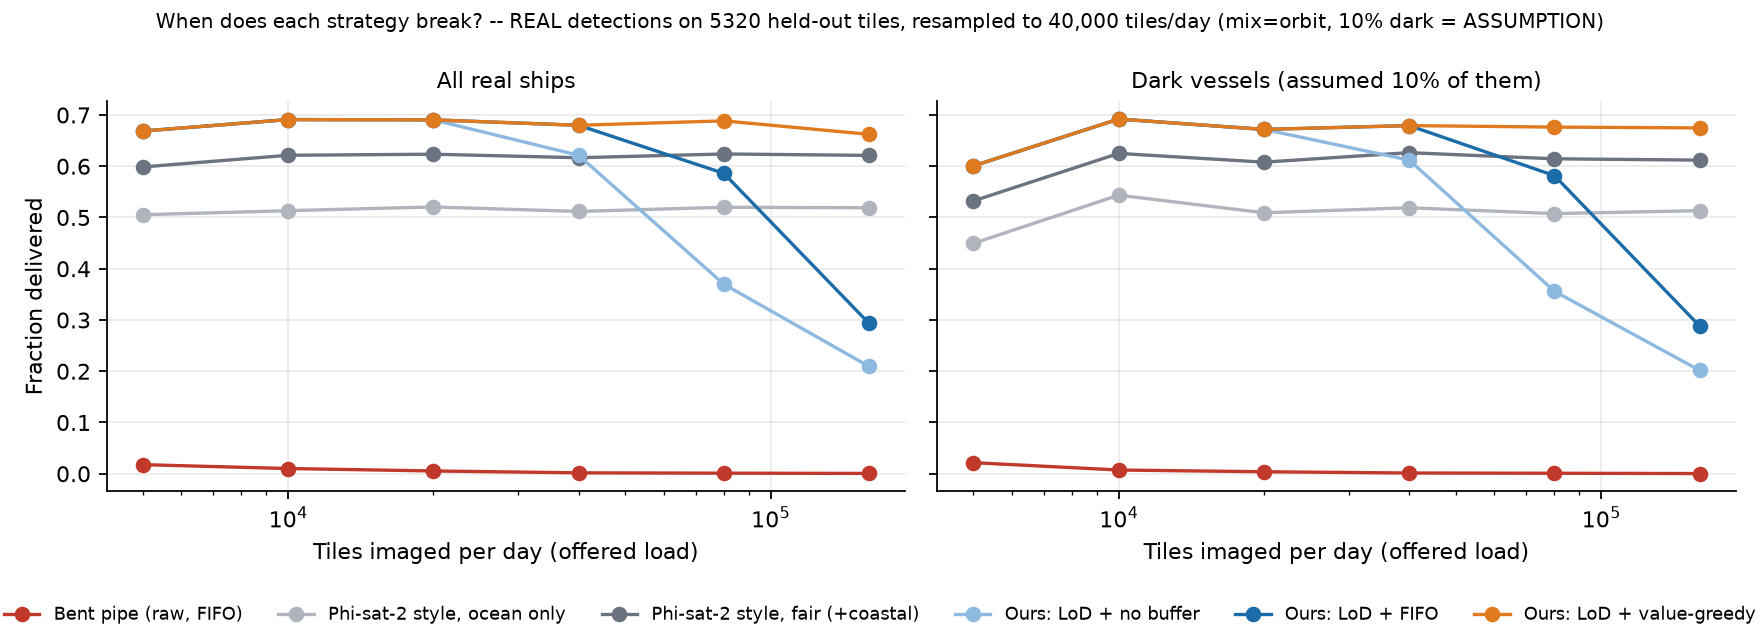
\includegraphics[width=0.9\textwidth]{wp6_real_sweep.png}
\caption{Recall against daily tile count \SIM. The three policies coincide until the link
saturates; past that, ordering by value per byte is what keeps recall flat.}\label{fig:sweep}
\end{figure}

\warnbox{\textbf{Correction to our own interim claim.} Our first Phi-sat-2 style baseline
encoded open-ocean patches only, so it ignored coastal ships \emph{by construction} --- a
comparison we were always going to win. Corrected, it scores $0.622$ rather than $0.518$, and our
advantage is $\mathbf{+6.3}$ points, not $+16.7$. A reviewer will check this; we would rather
state it than be caught by it.}

\subsection{Coupling the encoder to the queue}\label{sec:queue}

No fixed coastal policy is best in more than one load regime --- the optimum changes three times
between 20k and 320k tiles/day. Letting buffer pressure (queued bytes over capacity in the next
12 h, both quantities the satellite knows for free) slide the escalation threshold keeps us within
$1.1$ points of the best policy at \emph{every} load without being told the load. Worst-case
regret is $0.0058$ against $0.0123$ for the best fixed choice; the four fitted parameters were
re-run unchanged at two link budgets they were never tuned on. This is a \textbf{robustness}
result, not a higher peak, and we report it as such.

% =====================================================================
\section{How far from optimal?}\label{sec:opt}

The plan listed an optimality gap as a deliverable; no solver existed. We built an exact dynamic
program for the knapsack-with-concave-divisible-class, verified against brute-force enumeration
and bounded above by a fractional relaxation on every instance.

\begin{itemize}
\item \textbf{At operational scale greedy is essentially optimal}: $0.251\%$ mean gap. With
  $\sim$13{,}800 items of $\sim$1 kB in a 25--60 MB window the instance is nearly fractional, and
  greedy is exactly optimal for fractional knapsack.
\item \textbf{The gap is real only on lumpy windows}: $6.67\%$ mean, $54.8\%$ worst over saturated
  small instances. FIFO loses $67.3\%$ on the same queues.
\item \textbf{Over a whole day} the schedule sits within $7.1\%$ of a relaxation bound at the worst
  load, and \textbf{perfect foresight is worth at most $0.2\%$}. We therefore explicitly recommend
  \emph{against} building arrival prediction: against a perfect oracle the ceiling is one fifth of
  one percent.
\end{itemize}

% =====================================================================
\section{Failure modes, made executable}\label{sec:fmea}

Our interim FMEA table had eight entries, all prose; none of our 72 tests injected a fault. We
implemented 14 fault-injection tests, and the table failed in places.

The most serious: ``an AIS gap raises priority, not suspicion'' was \textbf{false for large
vessels}. Flagging a ship dark changed two things at once --- value $\times 5$ \emph{and} payload
L1$\to$L2. Because L2 grows as $\ell^{1.14}$ and L1 as $\ell^{0.57}$, above 128 px the extra bytes
outgrew the extra weight and a dark vessel ranked \emph{below} an identical ship with a clean AIS
track, on $13.6\%$ of real ships --- the largest ones. Decoupling the flag from the payload fixes
it by construction and is strictly better: large-dark recall $+24.1$ points, overall $+1.8$, dark
latency $-2.0$ h, for $+1.2\%$ bytes.

Two further claims did not hold as written: the thumbnail carries no ship identifiers, so it never
counts as delivery; and no watchdog exists. Both are now stated as gaps rather than mitigations.

% =====================================================================
\section{Which results depend on numbers we invented?}\label{sec:sens}

Seven unmeasured constants underpin every headline. Each was swept
(Figure~\ref{fig:tornado}). \textbf{Conclusions hold in 69 of 70 settings}; ``value-greedy
$\geq$ FIFO'' never fails. The single failure is $\texttt{thumb\_value}=0.1$, ten times baseline,
where thumbnails begin to crowd out ship chips --- so we state the constraint explicitly:
\texttt{thumb\_value} must stay below ${\sim}0.05$, and a two-dimensional sweep shows the binding
case is \emph{clear skies}, where more surviving ships compete for the link.

\begin{figure}[h]\centering
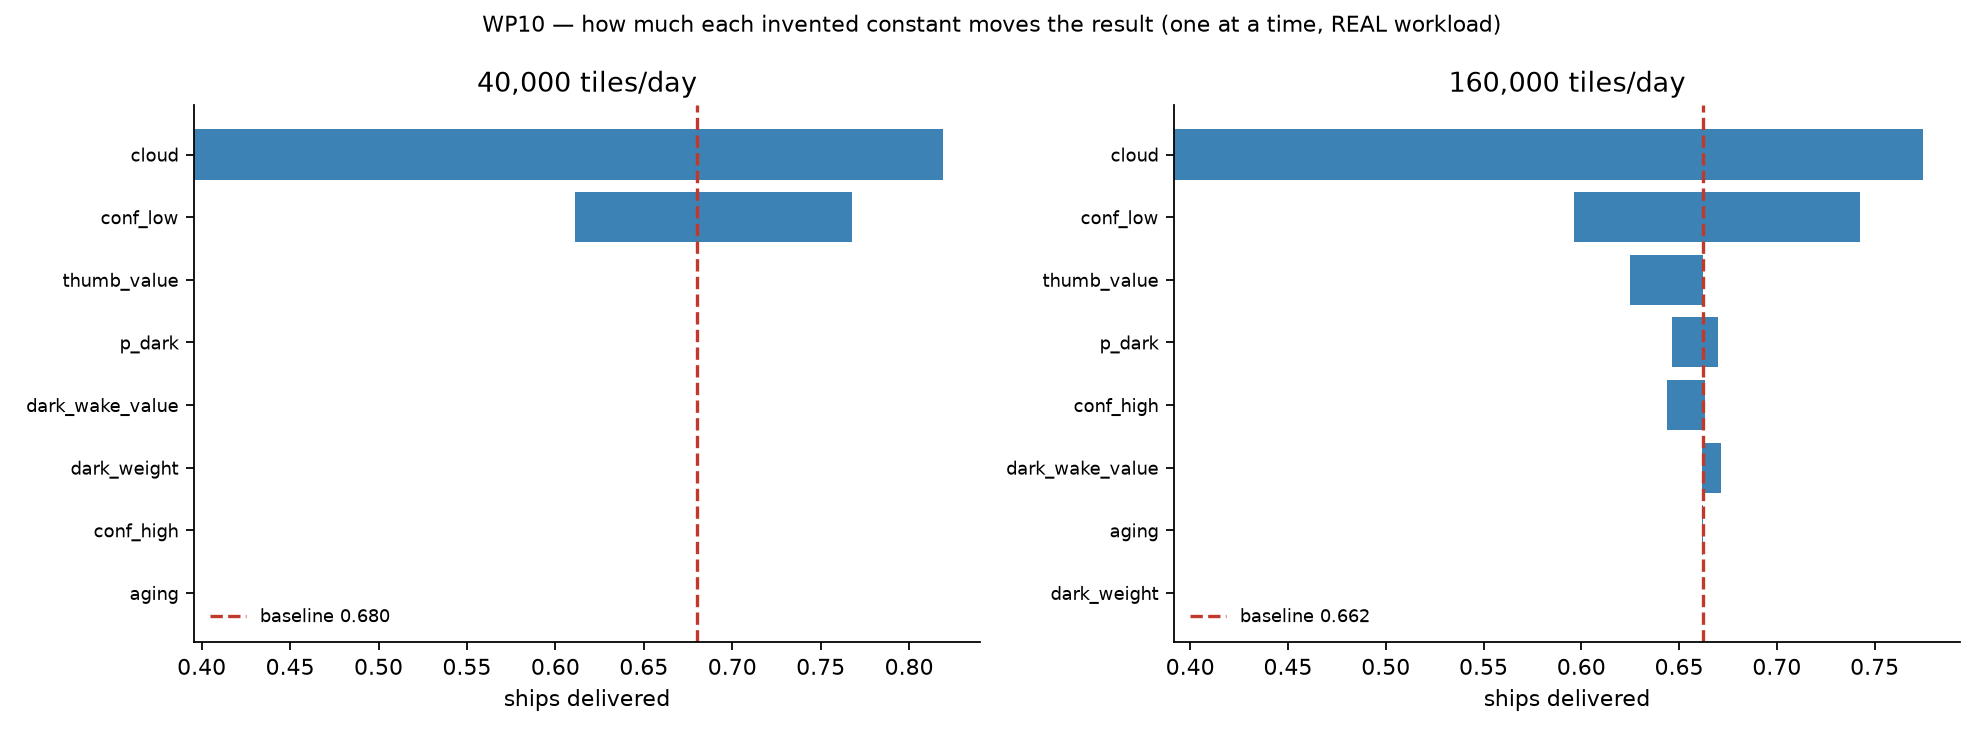
\includegraphics[width=0.78\textwidth]{wp10_tornado.png}
\caption{Sensitivity of ship recall to each invented constant \SIM. Cloud fraction dominates
everything else by roughly five times.}\label{fig:tornado}
\end{figure}

\warnbox{\textbf{The number we are least sure of is the loudest.} Cloud fraction has a recall
range of $0.42$ --- from $0.82$ at 0\% cloud to $0.40$ at 50\%. Worse, in our simulated day
6{,}025 cloud tiles are drawn from only \textbf{21 real cloudy tiles}, holding 12 real ships,
resampled $287\times$. Those 12 ships account for \textbf{52\% of everything we report as lost}.
We therefore never quote recall bare. The correct form is: \emph{0.685 at an assumed 15\% cloud
fraction; 0.40--0.82 across 0--50\%}. The Airbus set is $0.4\%$ cloud and cannot settle this; a
cloud climatology is required \LIT.}

% =====================================================================
\section{End-to-end validation}\label{sec:integration}

Sections~\ref{sec:results}--\ref{sec:sens} replay a stored catalogue rather than running the
models. We therefore ran the complete chain --- tile $\to$ pre-filter $\to$ gate $\to$ detector
$\to$ encoder $\to$ scheduler $\to$ ground --- on the full 5{,}320-tile test split from actual
JPEG bytes, and compared it tile by tile with the catalogue.

Context, tile class, candidate counts, ship counts and false alarms agree \textbf{exactly}. Ship
confidences differ in the last few digits (max $3\times10^{-4}$; different batch shapes select
different convolution kernels), and \textbf{one ship in 8{,}173} changes which prediction is
credited to it. The day-level result reproduces the simulation to four decimal places: 21{,}137
ships, 108.5 MB, recall $0.6798$ against $0.6799$. The replay is faithful.

\begin{figure}[h]\centering
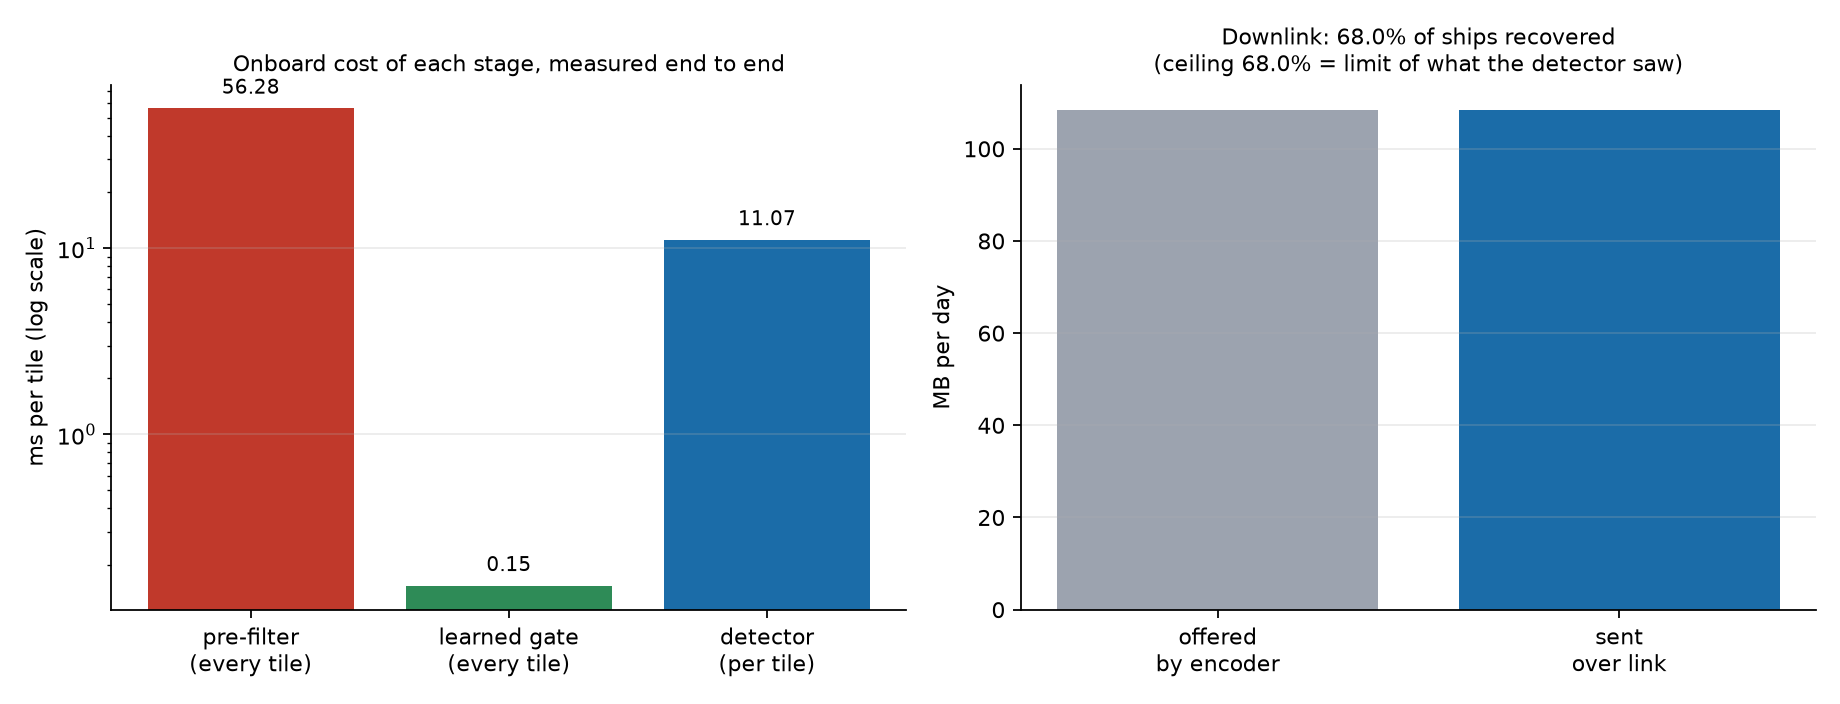
\includegraphics[width=0.9\textwidth]{wp11_funnel.png}
\caption{Measured on-board cost per stage, and the day's downlink \REAL. The classical
pre-filter costs $5.1\times$ the detector it is meant to gate.}\label{fig:funnel}
\end{figure}

% =====================================================================
\section{Tile seams: a decision we reversed on evidence}\label{sec:seams}

Our tiles arrive pre-cut at 768 px, so slicing-aided inference (SAHI \LIT) changes nothing here.
A real sensor produces a wide swath, and then every seam can cut a ship in half. On a
$10{,}000\times10{,}000$ px swath tiled at 768 px, a 200 px ship is cut $45.3\%$ of the time and a
380 px ship $74.5\%$ --- and large ships are the most valuable targets.

Geometry alone, however, overstates the problem. Measuring recall against the visible fraction of
a cut ship shows that \textbf{large ships barely notice}: at 50\% visible they are still detected
$0.915$ of the time, versus $0.101$ for small ships --- which are cut only $10.9\%$ of the time.
The two effects cancel, and the expected loss is $1.1\%$ to $7.5\%$ of ships, not $10$--$75\%$.

Comparing four policies on real tiles, an \emph{edge-triggered} scheme --- re-inference only where
the cheap stage sees an object touching a border --- \textbf{matches SAHI exactly} on seam recall
($0.875$ both) at $61\%$ of the compute. We therefore reject blanket SAHI and adopt edge-triggered
for Phase 3. The compute objection to SAHI has in any case disappeared: replacing the classical
pre-filter with the learned gate frees 56 ms/tile, roughly ten times what SAHI would spend.

% =====================================================================
\section{Limitations}\label{sec:limits}

Stated plainly, because several of them bound the claims above.

\begin{itemize}
\item \textbf{No flight hardware.} Every timing is a laptop RTX 5060. ``Runs on board'' is
  \emph{not} demonstrated, and this is the largest gap in the work.
\item \textbf{The cloud assumption dominates and is thinly evidenced} (Section~\ref{sec:sens}).
\item \textbf{Dark-vessel flags are assumed}, not measured; the Airbus data has no AIS.
\item \textbf{Tiles are resampled i.i.d.}, whereas a real pass sees correlated strips.
\item \textbf{One ground station.} The 11.4 h gap dominates latency.
\item \textbf{A quality setting we adopted as free is not.} Re-running the detector on
  recompressed coastal tiles shows the q60$\to$q40 move costs $4.0$ points of ship recall, all of
  it on small ships. The earlier measurement took recall from confidences computed on the
  \emph{original} file and could not have detected this. A further move to q30 is rejected on the
  same evidence.
\item \textbf{Small ships absorb every lossy step} --- INT8 quantisation, JPEG recompression and
  tile seams each take their toll there first. Small-ship recall is the single largest remaining
  loss in the system.
\end{itemize}

% =====================================================================
\section{Conclusion and Phase 3}

Spending a satellite's downlink on information rather than pixels reduces data volume
$557\times$ while delivering everything the satellite still knows about ships. The scheduler's
contribution is real but conditional: it is worth nothing until the link saturates, and worth
$2.26\times$ FIFO when it does. Greedy scheduling is within $0.251\%$ of optimal at our scale, and
clairvoyance is worth at most $0.2\%$ --- so the remaining engineering effort belongs in
\emph{detection}, not scheduling.

For Phase 3 we will: implement edge-triggered re-inference for wide swaths
(Section~\ref{sec:seams}); give the learned gate a localising head so the classical stage can be
removed entirely; obtain a cloud climatology to replace the assumption that currently dominates
our error bars; and attack small-ship recall, which every lossy stage in the pipeline punishes
first.

\paragraph{Reproducibility.} All code, all 15 work-package reports and every generated figure are
at \url{https://github.com/oblhdj/iastam-p7-semantic-downlink} under MIT. 96 automated tests cover
the encoder, scheduler, exact solver and 14 injected faults. The Airbus imagery is not
redistributed; a script rebuilds the leakage-free split from the original archive.

\paragraph{Tooling.} Development was assisted by Claude (Anthropic). Every experiment, number and
conclusion was specified, executed and reviewed by the team.

\end{document}
